\chapter {Problem setting}

\section {Channel model}

For simplicity we suppose uniform linear arrays, for which the response would be,
%
\DispNum {a:y':CN:NH} {
\V {a} \SB {\psi'}
= \frac {1} {\R {N_H}} \sum_{n_h=0}^{N_H-1} \mathsf {e} ^{\mathsf {i} n_h \psi'} \V {u} _{n_h}
\in \mathbb {C} ^ {N_H} 
}
%
where \m {\mathsf {e}} is the base of natural logarithm, and \m {\mathsf {i}} the imaginary unit.

And consider the virtual representation of the MIMO channel, as in Akdeniz et.\ al.\ \cite {ALS14},
%
\DispNum {H:H:l0:ql} {
\M {H}
=\sum_{l=0} ^{L-1}
\a_l
\V {a} \SB { 2\pi \frac {d_{\mathrm {arr}}} {\l _{\mathrm {arr}}} \sin \f_l'}
\V {a} \SB { 2\pi \frac {d_{\mathrm {arr}}} {\l _{\mathrm {arr}}} \sin \th_l'}^\dagger 
}
%
The physical meaning of \m {\f_l'} is the \m {l}-th angle of incidence (formed by the ray and the normal line) of departure electronic wave, and \m {\th_l'}, the \m {l}-th angle of arrival wave, and \m {d_{\mathrm {arr}}} is the distance between two adjacent antennae.
For our purpose, we may absorb the arguments of \m {\V {a}}
%
\DispNum {f:l:2p:2p} {
\f_l
= &2\pi \frac {d_{\mathrm {arr}}} {\l_{\mathrm {arr}}} \sin \f_l'
  \; \mathrm {Mod}\; \RB {2\pi} \\
%
\th_l
= &2\pi \frac {d_{\mathrm {arr}}} {\l_{\mathrm {arr}}} \sin \th_l'
  \; \mathrm {Mod}\; \RB {2\pi} 
}
%
to get a simpler form
%
\DispNum {H:H:l0:NH} {
\M {H}
=\sum_{l=0} ^{L-1} \a_l \V {a} \SB {\f_l} \V {a} \SB {\th_l}^\Adj
\in \mathbb {C} ^{N_H \D N_H} 
}


\section {System model}

\begin {figure} [hbt]
\centering
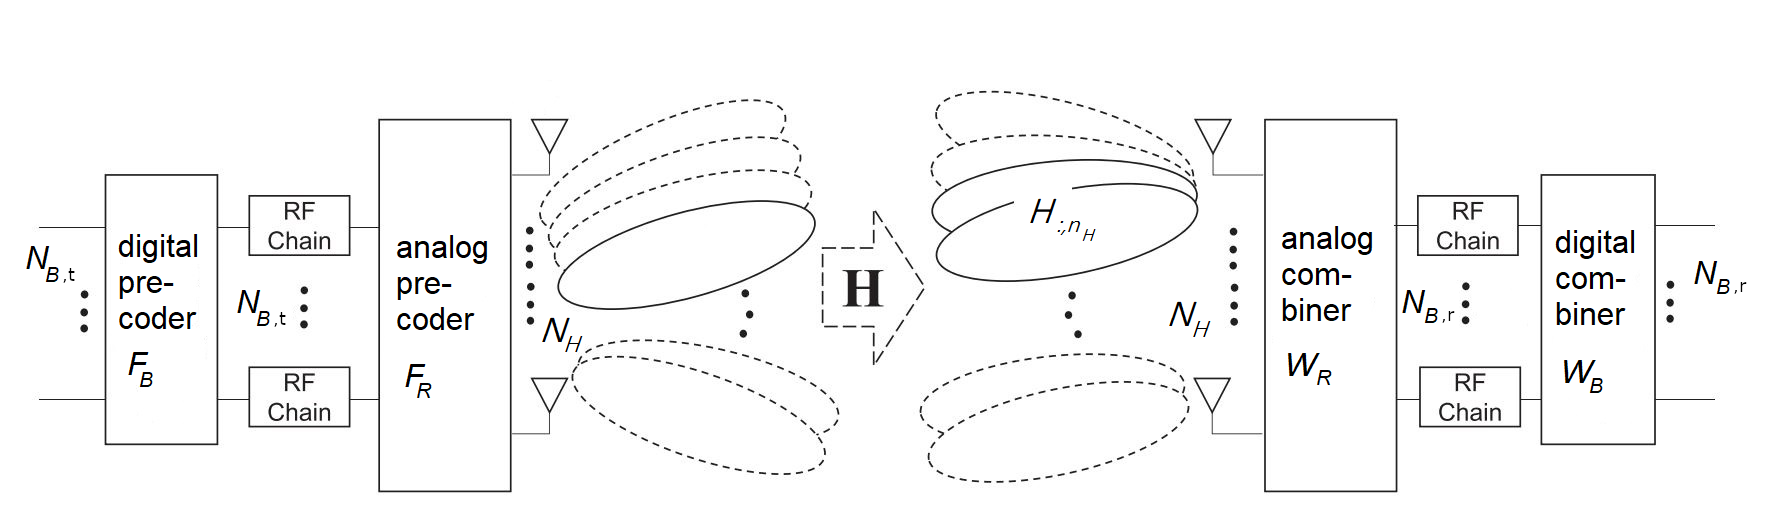
\includegraphics [width = \textwidth] {system.png}
\caption {Schematic diagram of the hybrid beamforming system we consider.}
\end {figure}

We consider the hybrid beamforming at both transmitter and receiver ends, as shown in Figure 2.
Each end consists of both digital and analog precoders and combiners.
In the transmitter end, there are (seeing towards the receiver end), digital precoder \m {\M {F} _B \in \mathbb {C} ^{N_{B,t} \D N_{B,t}}} and analog precoder \m {\M {F} _R \in \mathbb {C} ^{N_H \D N_{B,t}}}.
Similarly, in the receiver end, there are (seeing towards the transmitter end) digital combiner \m {\M {W} _R \in \mathbb {C} ^{N_{B,r} \D N_H}} and analog combiner \m {\M {W} _B \in \mathbb {C} ^{N_{B,r} \D N_{B,r}}}.

Recall that analog precoders may only have values of unity magnitude,
%
\DispNum {F:R:1::R1} {
\Nm {\RB {\M {F} _R} _{\SB {n_H, n_{R,t}}}}
= &1, \\
%
\Nm {\RB {\M {W} _R} _{\SB {n_{R,r}, n_H}}}
= &1, \\
%
n_H
= &0, \dots N_H-1, \\
%
n_{R,t}
= &0, \dots N_{B,t}-1  \\
%
n_{R,r}
= &0, \dots N_{B,r}-1 
}
%
And we assume
%
\DispNum {N:H:NY:NY} {
N_H \gg N_{B,t}, N_{B,r}
}

Since we restrict our discussion to a short interval of time, the noise term may be simply taken as a matrix \m {\M {Z} \in \mathbb {C} ^{N_H \D N_{B,t}}} with each entry being i.i.d.\ standard normal.
Let us introduce the effective channel
%
\DispNum {Y:Y:WB:BZ} {
\M {Y}
:=\M {W} _B \M {W} _R \RB {\M {H} \M {F} _R \M {F} _B +\M {Z}} 
}
%
Our task then amounts to recovering \m {\M {H}}, and generating \m {\M {W} _R}, \m {\M {W} _B}, \m {\M {F} _R}, and \m {\M {F} _B}.


\section {Vectorization}

We need several notations.
%
\Result
{Definition}
{
Define \m {\mathrm {vec} \SB {\M {A}} \in \mathbb {K} ^{N_1 \D N_2}} to be the vectorization of \m {\M {A} \in \mathbb {K} ^{N_1 \D  N_2}}.
Formally,
%
\DispNum {v:1:Am:N1} {
\RB {\mathrm {vec} \SB {\M {A}}} _{\SB {m}}
=\M {A} _{\SB {m\; \mathrm {Mod}\; N_1, \Fl {m/N_1 }}} 
}
%
The bijection is obvious, and we define \m {\mathrm {vec} ^{-1}} so that
%
\DispNum {v:x:x::x:} {
\mathrm {vec} ^{-1} \SB {\mathrm {vec} \SB {x}}
=x 
}
}

\Result
{Definition}
{
For \m {\M {A} \in \mathbb {K} ^{N_1 \D  N_2}} and \m {\M {B} \in \mathbb {K} ^{N_3 \D N_4}}, define the Kronecker product \m {\M {A} \otimes \M {B} \in \mathbb {K} ^{N_1 N_3 \D N_2 N_4}} by
%
\DispNum {A:2:Am:N4} {
&\RB {\M {A} \otimes \M {B}} _{\SB {m_1, m_2}} \notag \\
%
= &\M {A} _{\SB {\Fl {m_1/N_3 }, \Fl {m_2/N_4 }}}
\M {B} _{\SB {m_1\; \mathrm {Mod}\; N_3, m_2\; \mathrm {Mod}\; N_4}} 
}
}

The following relation, which is straightforward from definitions, is going be used below.
\Result
{Proposition}
{
Suppose \m {\M {A} \in \mathbb {K} ^{N_1 \D  N_2}, \M {X} \in \mathbb {K} ^{N_2 \D N_3}, \M {B} \in \mathbb {K} ^{N_3 \D N_4}},
Then
%
\DispNum {v:B:BA:cX} {
\mathrm {vec} \SB {\M {A}\M {X}\M {B}}
= \RB {\M {B}^\intercal \otimes \M {A}} \mathrm {vec} \SB {\M {X}} 
}
}

It is more appealing to write
%
\DispNum {h:h:ve:Nh} {
\V {h}
:= &\mathrm {vec} \SB {\M {H}}
\in \mathbb {C} ^{N_H^2} \\
%
\V {y}
:= &\mathrm {vec} \SB {\M {Y}}
\in \mathbb {C} ^{N_{B,t} N_{B,r}} \\
%
\V {z}
:= &\mathrm {vec} \SB {\M {W} _B \M {W} _R \M {Z}}
\in \mathbb {C} ^{N_{B,t} N_{B,r}} \\
%
\M {Q}
:= &\RB {\M {F} _B^\intercal \M {F} _R^\Tr} \otimes \RB {\M {W} _B \M {W} _R}
\in \mathbb {C} ^{N_{B,t} N_{B,r} \D N_H^2} 
}
%
to formulate the problem as a linear system:
%
\DispNum {y:y:Qh:hz} {
\V {y}
=\M {Q} \V {h} +\V {z} 
}
%
At this stage, we intend to apply DS, but there is no guarantee that \m {\V {h}} must be sparse.


\section {Spacial frequency domain}

Denote the discrete Fourier transform matrix to be \m {\M {K}},
%
\DispNum {K:K:CN:H1} {
\M {K} \in &\mathbb {C} ^{N_H \D N_H} \notag \\
%
\M {K} _{\SB {n_1, n_2}}
= &\frac {1} {\R {N_H}} \mathsf {e}^{2\pi \mathsf {i} n_1 n_2 /N_H}, \notag \\
%
\quad n_1, n_2
= &0, 1, \dots, N_H-1 
}
%
Recall that we have
%
\DispNum {K:K:I:::I} {
\M {K}^\dagger \M {K}
= \M {I} 
}
%
If we write
%
\DispNum {G:G:KH:HK} {
\M {G}
=\M {K}^\dagger \M {H} \M {K} 
}
%
then \m {\M {G}} can be interpreted as spatial frequency domain representation of \m {\M {H}}.
%
\DispNum {Y:Y:WB:NY} {
\M {Y}
=\M {W} _B \M {W} _R \M {K} \D \M {G} \D \M {K}^\dagger \M {F} _R \M {F} _B
+\M {W} _B \M {W} _R \M {Z}
\in \mathbb {C} ^{N_{B,r} \D N_{B,t}} 
}
%
If we are sure that \m {\M {G}} is sparse, then we recover \m {\M {G}} instead.
Set for brevity
%
\DispNum {P:P:FB:Nh} {
\M {P}
:=\RB {\M {F} _B^\intercal \M {F} _R^\intercal \M {K}^\ast} \otimes \RB {\M {W} _B \M {W} _R \M {K}}
\in \mathbb {C} ^{N_{B,t} N_{B,r} \D N_H^2} 
}
%
and
%
\DispNum {g:g:ve:Nh} {
\V {g}
:= \mathrm {vec} \SB {\M {G}}
\in \mathbb {C} ^ {N_H \D N_H} 
}
%
accordingly
%
\DispNum {y:y:Pg:gz} {
\V {y}
=\M {P} \V {g} +\V {z} 
}

\section {Proposed method}

Our plan becomes now

\Result
{Algorithm}
{
\begin {itemize}
%
\item Let \m {\g_{\mathrm {DS}} \geq 0} be given.
%
\item Input \m {\M {F} _B \in \mathbb {C} ^{N_R \D N_{B,t}}},
\m {\M {F} _R \in \mathbb {C} ^{N_H \D N_R}},
\m {\M {W} _R \in \mathbb {C} ^{N_R \D N_H}},
\m {\M {W} _B \in \mathbb {C} ^{N_{B,r} \D N_R}},
and \m {\M {Y} \in \mathbb {C} ^{N_{B,r} \D N_{B,t}}}.
%
\item Find \m {\M {P} \in \mathbb {C} ^{N_{B,r} N_{B,t} \D N_H^2}}, \m {\V {y} \in \mathbb {C} ^{N_H^2}} as in above.
%
\item Compute the convex program
%
\DispNum {g:g:mi:DS} {
\hat {\V {g}}
\leftarrow \begin {cases}
\Min {\V {g}' \in \mathbb {C} ^{N_H^2}} & \VNm {\V {g}'} _1 \\
%
\mathrm {subject} \; \mathrm {to} \quad & \VNm {\M {P}^\dagger \RB {\V {y} -\M {P} \V {g}'}} _\infty \leq \g_{\mathrm {DS}} \\
\end {cases} 
}
%
\item Convert \m {\hat {\V {g}}} back to the space domain, namely
%
\Disp {
\hat {\M {G}}
\leftarrow \mathrm {vec}^{-1} \SB {\hat {\V {g}}} 
}
%
\item Recover the estimated \m {\hat {\M {H}}}, as
%
\Disp {
\hat {\M {H}}
\leftarrow \M {K} \hat {\M {G}} \M {K}^\dagger 
}
%
\item Output \m {\hat {\M {H}}}.
%
\end {itemize}
}


